\documentclass[12pt]{article}
\usepackage[margin=2.5cm]{geometry}
\usepackage{enumerate}
\usepackage{amsfonts}
\usepackage{amsmath}
\usepackage{fancyhdr}
\usepackage{amsmath}
\usepackage{amssymb}
\usepackage{amsthm}
\usepackage{mdframed}
\usepackage{graphicx}
\usepackage{subcaption}
\usepackage{listings}
\usepackage{xcolor}
\usepackage[utf]{kotex}

\definecolor{codegreen}{rgb}{0,0.6,0}
\definecolor{codegray}{rgb}{0.5,0.5,0.5}
\definecolor{codepurple}{rgb}{0.58,0,0.82}
\definecolor{backcolour}{rgb}{0.95,0.95,0.92}

\lstdefinestyle{mystyle}{
    backgroundcolor=\color{backcolour},
    commentstyle=\color{codegreen},
    keywordstyle=\color{magenta},
    numberstyle=\tiny\color{codegray},
    stringstyle=\color{codepurple},
    basicstyle=\ttfamily\footnotesize,
    breakatwhitespace=false,
    breaklines=true,
    captionpos=b,
    keepspaces=true,
    numbers=left,
    numbersep=5pt,
    showspaces=false,
    showstringspaces=false,
    showtabs=false,
    tabsize=1
}

\lstset{style=mystyle}

\begin{document}
\title{CSC148 Worksheet 7 Solution}
\author{Hyungmo Gu}
\maketitle

\section*{Question 1}

\begin{itemize}
    \item Noticed that there are 11 students in total.
    \item Students should be grouped by year as closest as possible.
\end{itemize}

\bigskip

\textbf{Notes:}

\begin{itemize}
    \item 형모 해낼 뚜 있쬬!
    \item 형모 화이팅!
\end{itemize}

\section*{Question 2}
\begin{center}
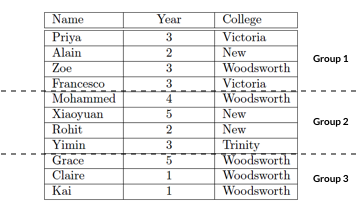
\includegraphics[width=0.7\linewidth]{images/worksheet_7_q2_solution.png}
\end{center}

\section*{Question 3}
\begin{itemize}
    \item

    First, we need to find the group as homogenous as possible in terms of year students
    are in.

    \bigskip

    The definition tells us group needs to be in 4,
    and the following table tell us there are 4 $3^{rd}$ year students.

    \bigskip

    \begin{center}
        \begin{tabular}{|c|c|}
            \hline
            Student Year & Number of Students\\
            \hline
            1 & 2\\
            \hline
            2 & 2\\
            \hline
            3 & 4\\
            \hline
            4 & 1\\
            \hline
            5 & 2\\
            \hline
        \end{tabular}
    \end{center}

    \bigskip

    It follows from these facts that the group of $3^{rd}$ year students best satisfy
    this criterion.

    \bigskip

    Next, we need to find the group as not homogenous as possible in terms of year students
    are in.

    \bigskip

    The same table tells us with 2 $5^{th}$ year students, 1 $4^{th}$
    year students and 1 $3^{rd}$ year student, a group spanning 3 years can be
    created.

    \bigskip

    Since we know there can't be a group spanning 4 years, we can conclude the
    group of 3 years (2 $5^{th}$ year students, 1 $4^{th}$ year students and 1
    $3^{rd}$ year student) best satisfy this criterion.

\end{itemize}

\bigskip

\begin{mdframed}
    \underline{\textbf{Correct Solution:}}

    \bigskip

    \color{red}
    Group 1 is the most homogeneous.

    \bigskip

    Group 3 is the least homogeneous.
    \color{black}

    \bigskip
\end{mdframed}

\bigskip

\section*{Question 4}
\begin{itemize}
    \item

    We will calculate the group score based on the code below. The code
    is also included in \textit{worksheet\_7\_q4\_solution.py}

    \bigskip

    \begin{lstlisting}[language=Python]
    def get_group_score(group):
        """Evaluates the group score

            Precondition: len(group) == 4
        """
        n = 4

        max_year = get_max_year(group)
        min_year = get_min_year(group)
        similarity_list = []

        i = 0

        while i < 4:
            j = 0
            while j < 4:
                # find the scaled distance
                scaled_distance = 0
                if max_year != min_year:
                    scaled_distance = abs(group[i]['year'] - group[j]['year']) / float(max_year - min_year)

                # find the similarity
                similarity = 1 - scaled_distance

                # add to list
                similarity_list.append(similarity)

                j += 1
            i += 1

        # find the average
        average = float(sum(similarity_list))/len(similarity_list)
        return average.as_integer_ratio()

    def get_max_year(group):
        """returns max value of year in group"""

        max_value = -1

        for student in group:
            max_value = max(student['year'], max_value)

        return max_value

    def get_min_year(group):
        """returns min value of year in group"""

        min_value = 100 # this is impossible value

        for student in group:
            min_value = min(student['year'], min_value)

        return min_value


    if __name__ == '__main__':
        group_1 = [{'name': 'Primya', 'year': 3},
        {'name': 'Zoe', 'year': 3},
        {'name': 'Francesco', 'year': 3},
        {'name': 'Yimin', 'year': 3}]

        group_2 = [{'name': 'Primya', 'year': 5},
        {'name': 'Zoe', 'year': 5},
        {'name': 'Francesco', 'year': 4},
        {'name': 'Yimin', 'year': 3}]


        score_1 =  get_group_score(group_1)
        print(score_1)

        score_2 =  get_group_score(group_2)
        print(score_2)


    \end{lstlisting}

    \bigskip

    For the most homogeneous group, the group score is 1.

    \bigskip

    For the least homogeneous group, the group score is $\frac{9}{16}$.

\end{itemize}

\bigskip

\begin{mdframed}
    \underline{\textbf{Correct Solution:}}

    \bigskip

    We will calculate the group score \color{red}using\color{black}\:the code below. The code
    is also included in \textit{worksheet\_7\_q4\_solution.py}

    \bigskip

    \begin{lstlisting}[language=Python]
    def get_similarity_list(group):
        """Evaluates the list of similarities""" # <- Correct solution
        similarity_list = []

        i = 0

        while i < len(group): # <- correct solution
            j = i + 1 # <- correct solution
            while j < len(group): # <- correct solution
                # find the scaled distance
                scaled_distance = abs(group[i]['year'] - group[j]['year']) / 5.0 # <- correct solution

                # find the similarity
                similarity = 1 - scaled_distance

                # add to list
                similarity_list.append(similarity)

                j += 1
            i += 1

        return similarity_list


    if __name__ == '__main__':
        # Correct Solution
        group_1 = [{'name': 'Primya', 'year': 3},
        {'name': 'Alain', 'year': 2},
        {'name': 'Zoe', 'year': 3},
        {'name': 'Francesco', 'year': 3}]

        # Correct Solution
        group_2 = [{'name': 'Mohammed', 'year': 4},
        {'name': 'Xiaoyuan', 'year': 5},
        {'name': 'Rohit', 'year': 2},
        {'name': 'Yimin', 'year': 3}]

        # Correct Solution
        group_3 = [{'name': 'Grace', 'year': 5},
        {'name': 'Claire', 'year': 1},
        {'name': 'Kai', 'year': 1}]

        # Correct Solution
        list_1 =  get_similarity_list(group_1)
        print(list_1)

        # Correct Solution
        list_2 =  get_similarity_list(group_2)
        print(list_2)

        # Correct Solution
        list_3 =  get_similarity_list(group_3)
        print(list_3)

    \end{lstlisting}

    \bigskip

    \color{red}
    We will calculate the score of each group in parts.

    \bigskip

    \underline{\textbf{Part 1 (Score of Group 1):}}

    \bigskip

    We need to calculate the score of group 1.

    \bigskip

    The problem tells us the group score is

    \begin{align}
        \text{Group Score} = \frac{\sum \text{similarities}}{\text{\# of elements in list of similarities}}
    \end{align}

    \bigskip

    and the above program tells us that the list of similarities are

    \begin{align}
        [0.8, 1.0, 1.0, 0.8, 0.8, 1.0]
    \end{align}

    \bigskip

    Then, using these facts, we can conclude that

    \begin{align}
        \text{Group Score} &= \frac{0.8 + 1.0 + 1.0 + 0.8 + 0.8 + 1.0}{6}\\
        &= \frac{\frac{4}{5} + 1 + 1 + \frac{4}{5} + \frac{4}{5} + 1}{6}\\
        &= \frac{\frac{4}{5} + \frac{5}{5} + \frac{5}{5} + \frac{4}{5} + \frac{4}{5} + \frac{5}{5}}{6}\\
        &= \frac{\frac{27}{4}}{6}\\
        &= \frac{27}{30}\\
        &= \frac{9}{10}
    \end{align}

    \bigskip

    \underline{\textbf{Part 2 (Score of Group 2):}}

    \bigskip

    We need to calculate the score of group 2.

    \bigskip

    The problem tells us the group score is

    \begin{align}
        \text{Group Score} = \frac{\sum \text{similarities}}{\text{\# of elements in list of similarities}}
    \end{align}

    \bigskip

    and the above program tells us that the list of similarities are

    \begin{align}
        [0.8, 0.6, 0.8, 0.4, 0.6, 0.8]
    \end{align}

    \bigskip

    Then, we can conclude that the value of group score is

    \begin{align}
        \frac{0.8 + 0.6 + 0.8 + 0.4 + 0.6 + 0.8}{6} &= \frac{\frac{4}{5} + \frac{3}{5} + \frac{4}{5} + \frac{2}{5} + \frac{3}{5} + \frac{4}{5}}{6}\\
        &= \frac{\frac{20}{5}}{6}\\
        &= \frac{20}{30}\\
        &= \frac{2}{3}
    \end{align}

    \bigskip

    \underline{\textbf{Part 3 (Score of Group 3):}}

    \bigskip

    We need to calculate the score of group 3.

    \bigskip

    The problem tells us the group score is

    \begin{align}
        \text{Group Score} = \frac{\sum \text{similarities}}{\text{\# of elements in list of similarities}}
    \end{align}

    \bigskip

    and the above program tells us that the list of similarities are

    \begin{align}
        [0.2, 0.2, 1.0]
    \end{align}

    \bigskip

    Then, we can conclude that the value of group score is

    \begin{align}
        \frac{0.2 + 0.2 + 1.0}{3} &= \frac{\frac{1}{5} + \frac{1}{5} + \frac{5}{5}}{3}\\
        &= \frac{\frac{7}{5}}{3}\\
        &= \frac{7}{15}
    \end{align}

    \color{black}
\end{mdframed}

\bigskip

\textbf{Notes:}

\begin{itemize}
    \item Realized that `group' in question means `group 1`, `group 2` and `group 3' in question 2 :(.
\end{itemize}

\bigskip

\section*{Question 5}
\begin{itemize}
    \item

    \bigskip

    We need to find the highest and the lowest possible score on this criterion.

    \bigskip

    We will do so in parts.

    \bigskip

    \underline{\textbf{Part 1 (Calculating highest possible group score):}}

    \bigskip

    We need to find the highest possible group score on this criterion.

    \bigskip

    The definition of group score tells us that

    \setcounter{equation}{0}
    \begin{align}
        \text{Group Score} = \frac{\displaystyle\sum\limits_{i=0}^{n-1} \displaystyle\sum\limits_{j=i+1}^{n-1} \left(1 - \displaystyle\frac{\lvert student\_year_i - student\_year_j \rvert}{5} \right)}{\text{\# of elements in list of similarities}}
    \end{align}

    \bigskip

    By observation, we can conclude that the highest possible group score happens when
    $\lvert student\_year_i - student\_year_j \rvert = 0$.

    \bigskip

    Then, using this fact, we can calculate that

    \begin{align}
        \text{Group Score} &= \frac{\displaystyle\sum\limits_{i=0}^{n-1} \displaystyle\sum\limits_{j=i+1}^{n-1} \left(1 - \displaystyle\frac{\lvert student\_year_i - student\_year_j \rvert}{5} \right)}{\text{\# of elements in list of similarities}}\\
        &= \frac{\displaystyle\sum\limits_{i=0}^{n-1} \displaystyle\sum\limits_{j=i+1}^{n-1} 1}{\text{\# of elements in list of similarities}}
    \end{align}

    \bigskip

    Then, because we know $\sum\limits_{i=0}^{n-1}\sum\limits_{j=i+1}^{n-1} 1 = \text{\# of elements in list of similarities}$,
    we can conclude

    \begin{align}
        &= \frac{\text{\# of elements in list of similarities}}{\text{\# of elements in list of similarities}}\\
        &= 1
    \end{align}

    \bigskip

    \underline{\textbf{Part 2 (Calculating lowest possible group score):}}

    \bigskip

    We need to find the lowest possible group score achievable on this criterion.

    \bigskip

    The definition of group score tells us that

    \begin{align}
        \text{Group Score} = \frac{\displaystyle\sum\limits_{i=0}^{n-1} \displaystyle\sum\limits_{j=i+1}^{n-1} \left(1 - \displaystyle\frac{\lvert student\_year_i - student\_year_j \rvert}{5} \right)}{\text{\# of elements in list of similarities}}
    \end{align}

    \bigskip

    By observation, we can conclude that the lowest possible group score happens when
    $\lvert student\_year_i - student\_year_j \rvert = 5$.

    \bigskip

    Then, using this fact, we can calculate that

    \begin{align}
        \text{Group Score} &= \frac{\displaystyle\sum\limits_{i=0}^{n-1} \displaystyle\sum\limits_{j=i+1}^{n-1} \left(1 - \displaystyle\frac{\lvert student\_year_i - student\_year_j \rvert}{5} \right)}{\text{\# of elements in list of similarities}}\\
        &= \frac{\displaystyle\sum\limits_{i=0}^{n-1} \displaystyle\sum\limits_{j=i+1}^{n-1} 0}{\text{\# of elements in list of similarities}}\\
        &= \frac{0}{\text{\# of elements in list of similarities}}\\
        &= 0
    \end{align}
\end{itemize}

\bigskip

\textbf{Notes:}

\begin{itemize}
    \item 형모야. 차분히. 한걸음 더.
    \item 문제 안풀린다고 주저 앉지마.
    \item 사랑하는 내 여보 향해 가는거야.
    \item 보고싶은 내 여보 향해.
    \item 형모야 화이팅 :)
\end{itemize}

\section*{Question 6}

\begin{center}
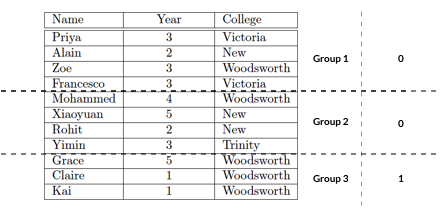
\includegraphics[width=0.7\linewidth]{images/worksheet_7_q6_solution.png}
\end{center}

\section*{Question 7}

\section*{Question 8}

\section*{Question 9}

\section*{Question 10}

\end{document}